% This Latex poster uses the baposter class, originally from
% http://www.brian-amberg.de/uni/poster. Versions are found in several places.
% The files on which this version is based are from circulation within WASP
% and exact origins are not known.
%
% CONTENT
% To update the poster, modify the contents in the parts/ folder.
% The file header.tex contains convenience commands such as \title, \companylogo etc.
% Other files contain pure formatting.
%
% COLORS
% The following standard colors are defined: wasp_text, wasppink, waspgrey, waspblue
%
% Enjoy!
% Per Skarin, 2021

\documentclass[a0paper,portrait]{baposter}
\usepackage{lipsum}  
\usepackage[square, numbers, comma, sort&compress]{natbib}  % Use the "Natbib" style for the references in the Bibliography
\usepackage{relsize}	% For \smaller
\usepackage{url}	% For \url
\usepackage{epstopdf}	% Included EPS files automatically converted to PDF to include with pdflatex
\usepackage[utf8]{inputenc} 
\usepackage{multirow}
\usepackage{booktabs}
\usepackage[labelfont=bf]{caption}
\usepackage{enumitem}
\usepackage{tcolorbox}
\usepackage{mathtools}
\usepackage{multicol}
\usepackage{setspace}
\usepackage{float}
\usepackage[font=footnotesize,skip=3pt,justification=raggedright,singlelinecheck=false]{caption}
\usepackage{subcaption}
\usepackage[super]{nth}

% \setstretch{0.85}

% PATHS
\graphicspath{{template-images/}{content-images/}}

% FONTS AND COLORS
\renewcommand{\familydefault}{\sfdefault}
\newcommand{\mytitlefont}{\fontfamily{\familydefault}\selectfont }
\newcommand{\mytextfont}{\fontfamily{\familydefault}\selectfont }
% Comment the four lines below to skip WASP fonts
%\usepackage{MinionPro}
%\usepackage{MyriadPro}
% \renewcommand{\mytitlefont}{\fontfamily{MyriadPro-LF}\selectfont }
% \renewcommand{\mytextfont}{\fontfamily{MinionPro-LF}\selectfont }

\definecolor{wasppink}{RGB}{203,166,169} 
\definecolor{waspgrey}{RGB}{88,89,91}
\definecolor{wasplgrey}{RGB}{188,188,188}
\definecolor{waspblue}{RGB}{26,141,173}
\definecolor{darkgreen}{rgb}{0,0.6,0}

\definecolor{wasp_text}{RGB}{66,80,82}
\colorlet{wasp_banner_light}{waspblue}
\colorlet{wasp_banner_dark}{wasplgrey}

% LIST SETTINGS
\setlist{itemsep=.1em, leftmargin=1em}

% COMMANDS
\newcommand\thetitle{}\renewcommand\title[1]{\renewcommand\thetitle{#1}}
\newcommand\theauthor{}\renewcommand\author[1]{\renewcommand\theauthor{#1}}
\newcommand\thedepinfo{}\newcommand\depinfo[1]{\renewcommand\thedepinfo{#1}}
\newcommand\thesupervisors{}\newcommand\supervisors[1]{\renewcommand\thesupervisors{#1}}
\newcommand\theuniversitylogo{}\newcommand\universitylogo[1]{\renewcommand\theuniversitylogo{#1}}
\newcommand\thecompanylogo{}\newcommand\companylogo[1]{\renewcommand\thecompanylogo{#1}}


%%%%%%%%%%%%%%%%%%%%%%%%%%%%%%%%%%%%%%%%%%%%%%%%%%%%%%%%%%%%%%%%%%%%%%%%%%%%%%%
%%% Document Start %%%%%%%%%%%%%%%%%%%%%%%%%%%%%%%%%%%%%%%%%%%%%%%%%%%%%%%%%%%%
%%%%%%%%%%%%%%%%%%%%%%%%%%%%%%%%%%%%%%%%%%%%%%%%%%%%%%%%%%%%%%%%%%%%%%%%%%%%%%%

% Text to the left
\title{Methanogenic Archaeal Class Bog-38 In the North Selangor Peat Swamp Forest: A Tropical Outlier In a Predominantly Arctic Lineage}
\author{Muhammad Zarul Hanifah Md Zoqratt\textsuperscript{a} Patrick Hock Siew Tan\textsuperscript{a}, Vanessa Wong\textsuperscript{b}, Adzzie Shazleen Azman\textsuperscript{a}, Holly Barclay\textsuperscript{a}, Qasim Ayub\textsuperscript{a,c}}
\depinfo{\textsuperscript{a}School of Science, Monash University Malaysia, Bandar Sunway, Selangor, 47500, Malaysia
         \textsuperscript{b}School of Earth, Atmosphere and Environment, Monash University, Clayton, VIC, Australia
         \textsuperscript{c}Monash University Malaysia Genomics Platform, Bandar Sunway, Selangor Darul Ehsan, 47500, Malaysia
         }
% \supervisors{}

% Logos on the right. Put the images in template-images/

\universitylogo{
\includegraphics[width=0.7\textwidth]{template-images/university/Monash.png}}
\companylogo{\includegraphics[width=0.7\textwidth]{company/ericsson}}



\begin{document}

%%% General Poster Settings %%%%%%%%%%%%%%%%%%%%%%%%%%%%%%%%%%%%%%%%%%%%%%%%%%%
%%%%%% Eye Catcher, Title, Authors and University Images %%%%%%%%%%%%%%%%%%%%%%
\begin{poster}{
 % Show grid to help with alignment
 grid=false,
 eyecatcher=true,
 % Column spacing
 colspacing=0.5em,
 columns=3,
 boxpadding=.2cm,
 % Color style
 headerColorOne=wasp_banner_light,
 borderColor=wasp_banner_light,
 headerFontColor=cyan!10!white,
 % Format of textbox
 textborder=faded,
 % Format of text header
 headerborder=open,
 headershape=roundedright,
 headershade=plain,
 background=none,
 % bgColorOne=cyan!10!white,
 headerheight=0.06\textheight}
%%% Eye Cacther %%%%%%%%%%%%%%%%%%%%%%%%%%%%%%%%%%%%%%%%%%%%%%%%%%%%%%%%%%%%%%%
{
	Eye Catcher, empty if option eyecatcher=false - unused
}
%%%% Title %%%%%%%%%%%%%%%%%%%%%%%%%%%%%%%%%%%%%%%%%%%%%%%%%%%%%%%%%%%%%%%%%%%%%
{
	\textcolor{wasp_text}{\mytitlefont \large \thetitle}
}
%%% Authors %%%%%%%%%%%%%%%%%%%%%%%%%%%%%%%%%%%%%%%%%%%%%%%%%%%%%%%%%%%%%%%%%%%
{
  \vspace{0.1em}
  \textcolor{wasp_text}{\footnotesize \theauthor\\
	% \normalsize Supervisors: \thesupervisors\\
	\thedepinfo\\
	}
}
%%% Logo %%%%%%%%%%%%%%%%%%%%%%%%%%%%%%%%%%%%%%%%%%%%%%%%%%%%%%%%%%%%%%%%%%%%%%
{
  \begin{minipage}{4.5cm}
   \centering
   % \righting
   \vspace{0.5cm}
            
	    \theuniversitylogo\vspace{0.25cm}\par
		  % \thecompanylogo
  \end{minipage}
}

%%%%%%%%%%%%%%%%%%%%%%%%%%%%%%%%%%%%%%%%%%%%%%%%%%%%%%%%%%%%%%%%%%%%%%%%%%%%%%
%%% Now define the boxes that make up the poster
%%%---------------------------------------------------------------------------
%%% Each box has a name and can be placed absolutely or relatively.
%%% The only inconvenience is that you can only specify a relative position 
%%% towards an already declared box. So if you have a box attached to the 
%%% bottom, one to the top and a third one which should be inbetween, you 
%%% have to specify the top and bottom boxes before you specify the middle 
%%% box.
%%%%%%%%%%%%%%%%%%%%%%%%%%%%%%%%%%%%%%%%%%%%%%%%%%%%%%%%%%%%%%%%%%%%%%%%%%%%%%
% \headerbox{t}{column=0,row=0,span=1}{}
%%%%%%%%%%%%%%%%%%%%%%%%%%%%%%%%%%%%%%%%%%%%%%%%%%%%%%%%%%%%%%%%%%%%%%%%%%%%%%
  \headerbox{\mytitlefont Introduction}{name=introduction,column=0,row=0,span=3}{
  \mytextfont
%%%%%%%%%%%%%%%%%%%%%%%%%%%%%%%%%%%%%%%%%%%%%%%%%%%%%%%%%%%%%%%%%%%%%%%%%%%%%%
  % Put the motivation behind and goals of the research here
\footnotesize
% \lipsum[2]

{\setstretch{0.85}

\textbf{Introduction:} The archaeal class Bog-38 has been predominantly associated with cold-region peatlands, particularly across Arctic and sub-Arctic permafrost ecosystems, where it contributes to methane production. However, its presence and role in tropical environments remain poorly understood. \textbf{Methods:} To investigate the potential distribution and function of Bog-38 in tropical ecosystems, peat soil samples were collected from four distinct sites within the North Selangor Peat Swamp Forest (NSPSF), Peninsular Malaysia. Five different depths were sampled at each site. DNA was extracted from these samples and sequenced using the Oxford Nanopore P2 Solo platform to generate long-read metagenomic data. \textbf{Results and Discussion:} Twelve Bog-38 metagenome-assembled genomes (MAGs) were recovered, with at least three assembled as complete circular genomes. These tropical MAGs contained key methanogenesis genes—mcrA, mcrB, and mcrG—encoding the methyl-coenzyme M reductase (MCR) complex, essential for methane biosynthesis. Comparative phylogenomic analysis revealed that the NSPSF Bog-38 MAGs form distinct clades, indicating significant phylogenetic divergence from Arctic counterparts. Functional profiling of the tropical MAGs also suggested unique metabolic adaptations potentially relevant to the anaerobic, lignin-rich environment of tropical peat soils. \textbf{Conclusion:} These findings expand the known geographic and functional diversity of Bog-38, establishing tropical peatlands like the NSPSF as important reservoirs of novel methanogenic archaea. This challenges previous assumptions of their restriction to permafrost ecosystems and highlights the broader ecological relevance of tropical methane-cycling communities.
}
}

%%%%%%%%%%%%%%%%%%%%%%%%%%%%%%%%%%%%%%%%%%%%%%%%%%%%%%%%%%%%%%%%%%%%%%%%%%%%%%
  \headerbox{\mytitlefont Methods}{name=methods,column=0,row=0,span=1, below=introduction}{
%%%%%%%%%%%%%%%%%%%%%%%%%%%%%%%%%%%%%%%%%%%%%%%%%%%%%%%%%%%%%%%%%%%%%%%%%%%%%%
  \mytextfont
  % The methods that you use goes here

\footnotesize

The NSPSF is the largest remaining peatland in Peninsular Malaysia, located in northwestern Selangor near the coastal town of Sekinchan, covering ~81,304 hectares (Figure \ref{fig:map}). The land was originally logged in the 1930s and later gazetted as a protected area in the 1990s \cite{GEC_2014}. To the west lies a paddy field, part of the Tanjong Karang Irrigation Scheme, which receives drainage from the forest. Surrounding land uses include oil palm plantations, rehabilitated logging zones, and protected forest areas managed by the Selangor Forestry Department.

Entry and sampling were conducted under research permit JH/100 Jld. 31 (59), with additional approvals from the Klang and Rawang District Forestry Offices.

\begin{figure}[H]
    \vspace{-0.4cm}
    \centering
    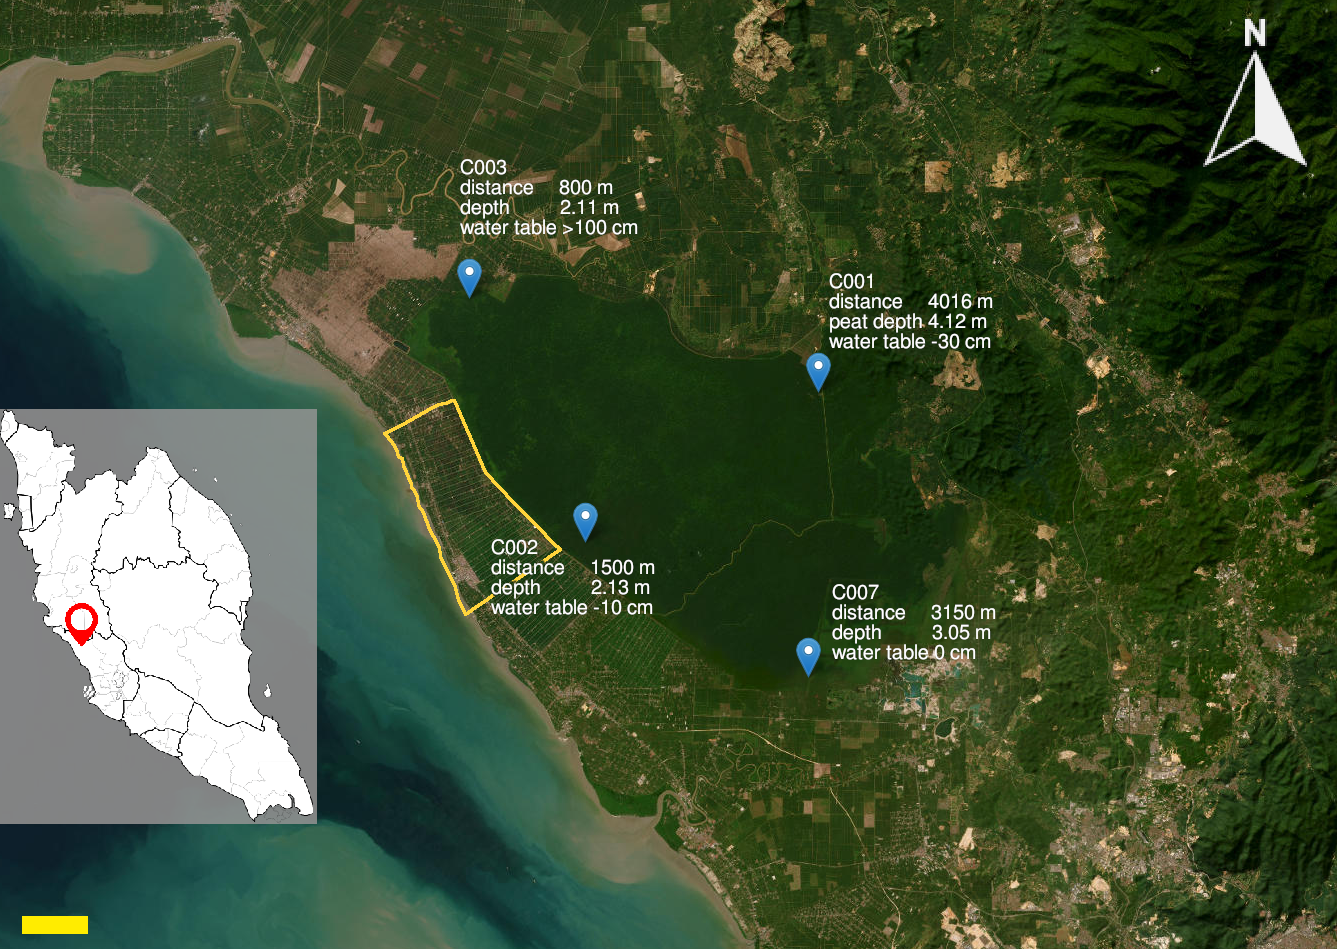
\includegraphics[width=0.9\linewidth]{content-images/map_plot4.png}
    \caption{\scriptsize Map of the NSPSF, Selangor, Peninsular Malaysia. The four sampling sites are marked with blue indicators. The scale bar in the bottom left represents a distance of 5 kilometers. The yellow boundary outlines the nearby town of Sekinchan and surrounding paddy fields. The inset map shows the location of the NSPSF (red marker) within Peninsular Malaysia.}
    \label{fig:map}
\end{figure}

\vspace{-0.3cm}

We collected 20 peat soil samples representing four contrasting NSPSF sites, each sampled at five distinct depths across the peat profile (Figure \ref{fig:map}). Genomic DNA was extracted from peat soil using a modified protocol involving cryogenic grinding, chemical lysis, and purification with chloroform:isoamyl alcohol, ethanol precipitation, and AMPure XP bead cleanups. DNA quality was evaluated via NanoDrop and Qubit. Libraries were prepared using the SQK-LSK114 ligation kit and sequenced on FLO-PRO114M flow cells with the Oxford Nanopore P2 Solo platform. We generated a minimum of 80 Gb of sequencing data per sample to ensure sufficient coverage for capturing low-abundance taxa, including methanogens.

Bioinformatics analyses were performed using the M3 MASSIVE HPC cluster (Victoria, Australia) and the Advanced Computing Platform (Monash Malaysia). The workflow is summarized in Figure \ref{fig:workflow}, and full details and workflows are available at: \url{github.com/ZarulHanifah/8thICMBB2025} \cite{Kolmogorov_2019_flye, Alneberg_2014_concoct, Pan_2022_semibin, Mallawaarachchi_2022_metacoag, Shaffer_2020_dram}.

\begin{figure}[H]
    \vspace{-0.4cm}
    \centering
    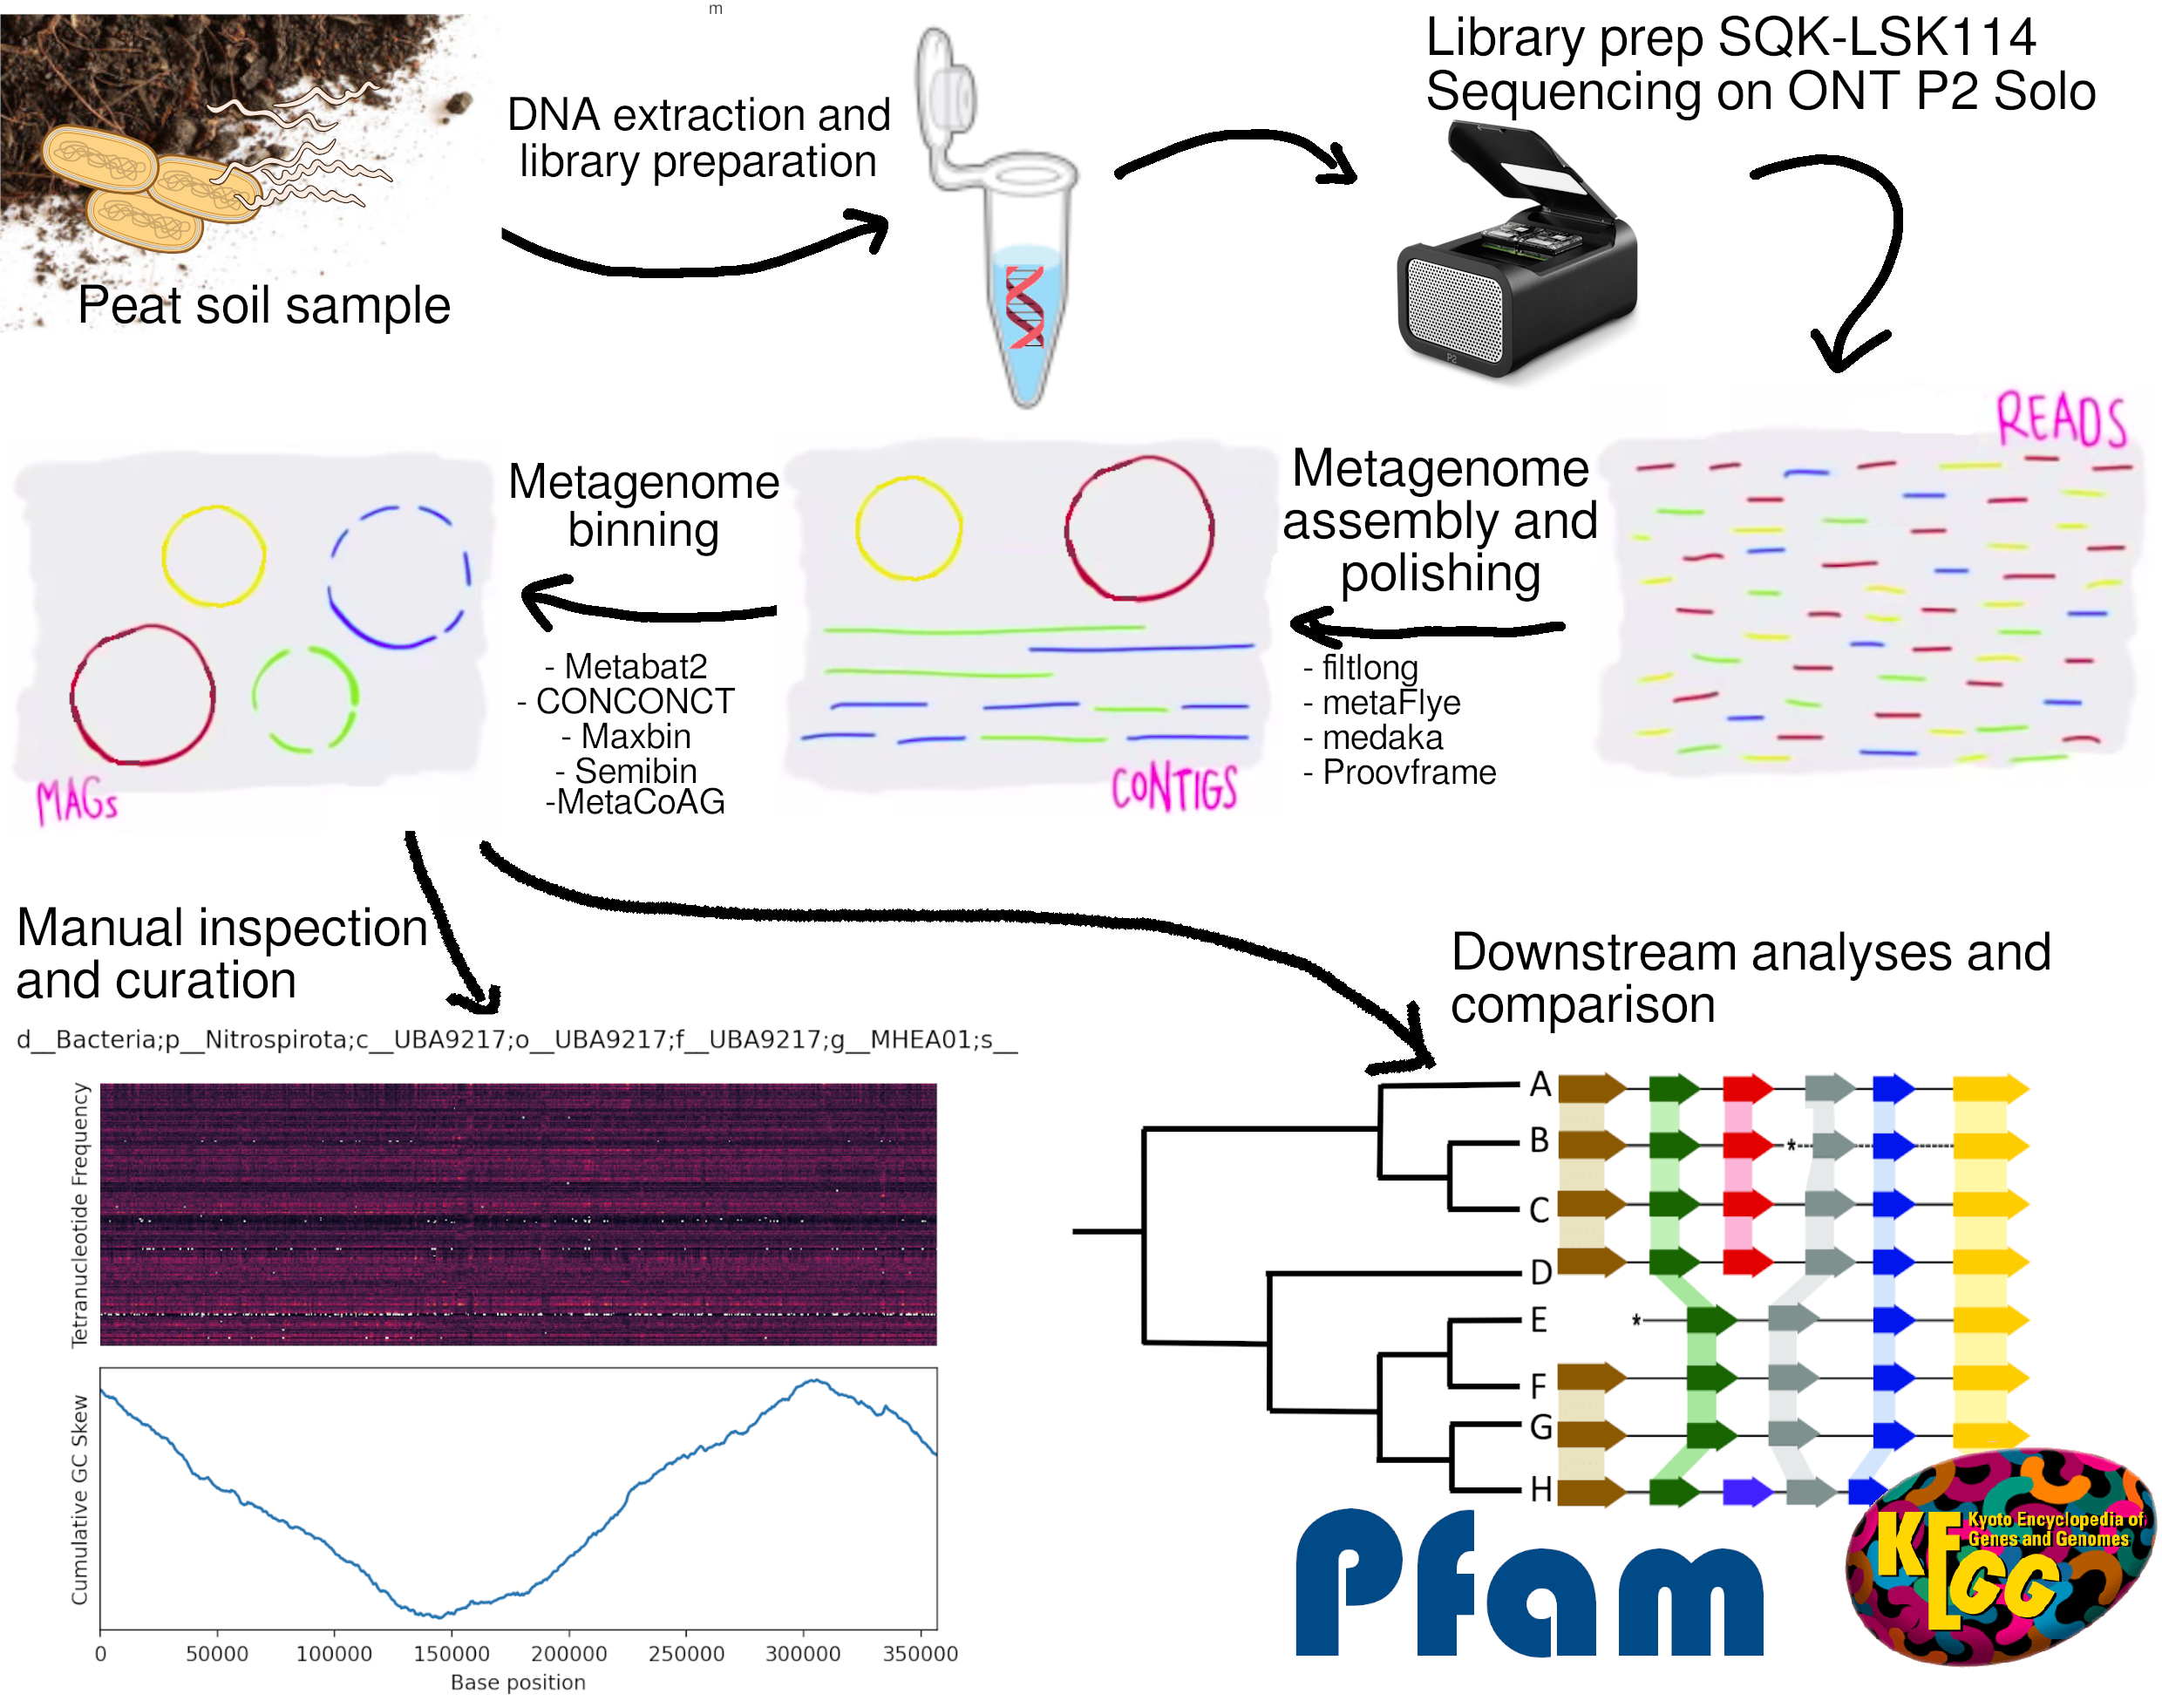
\includegraphics[width=0.9\linewidth]{experimental_design}
    \caption{\scriptsize Flowchart summarizing the workflow DNA extraction, sequencing on Oxford Nanopore P2 Solo platform and bioinformatics analyses. Manual curation and inspection included genome circulation and reorientation, and display of tetranucleotide frequency and GC skew.}
    \label{fig:workflow}
\end{figure}

% \vspace{2em} % Fill in to put references at the bottom

}

%%%%%%%%%%%%%%%%%%%%%%%%%%%%%%%%%%%%%%%%%%%%%%%%%%%%%%%%%%%%%%%%%%%%%%%%%%%%%%
  \headerbox{\mytitlefont Results and Discussions}{name=results,column=1,row=0,span=2, below=introduction }{
%%%%%%%%%%%%%%%%%%%%%%%%%%%%%%%%%%%%%%%%%%%%%%%%%%%%%%%%%%%%%%%%%%%%%%%%%%%%%%
  \mytextfont
  \footnotesize
\begin{multicols}{2}[\columnsep=0.4cm]
    Methanogenic activity requires lab enrichment and methanogenic activity validation, therefore putative methanogens and methanotrophs are addressed as MCR-encoding MAGs.

    \vspace{0.2cm}
    
    MCR-encoding MAGs are found in the NSPSF dataset, belonging to taxonomic groups c\_\_Bog-38 (class Bog-38, according to GTDB release 220) \cite{Chaumeil_2022_gtdbtk}, f\_\_JACTUA01, g\_\_ANME-1-THS, g\_\_Methanobacterium\_A and f\_\_JACAEJ01. Bog-38 demonstrated the highest abundance amongst MCR-encoding MAGs, as well being highly prevalent across different sites, although mostly absent at the surface.

    \begin{figure}[H]
        \vspace{-0.4cm}
        \centering
        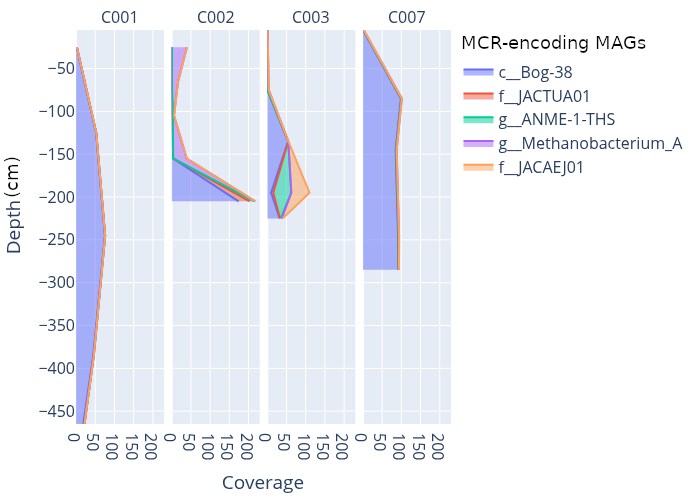
\includegraphics[width=\linewidth]{content-images/abundance_depth.png}
        \caption{\scriptsize Coverage of MCR-encoding archaeal groups across sampling sites and depths. Coverage refers to the average sequencing depth of each MAG, calculated as the mean number of reads mapped per base pair of the genome, providing an estimate of its relative abundance in the sample.}
        \label{fig:coverage}
    \end{figure}  

    \vspace{-0.4cm}
    
    We constructed a Bog-38 maximum likelihood phylogenomic tree from concatenation of 76 single-copy core genes, consisting of MAGs from the NSPSF dataset as well as from the Genome Taxonomy Database (GTDB) release 220 (Figure \ref{fig:phylo}) \cite{Lee_2019_gtotree}. Inclusion of NSPSF MAGs contributed immensely in phylogenetic gain of Bog-38 by 73.4\%. Several NSPSF MAGs form unique clades, where these MAGs cluster away from GTDB MAGs. Almost 90\% of these GTDB MAGs originate from shotgun metagenomic projects of the Stordalen Mire in Sweden, and are taxonomically associated to \emph{Methanoflorens stordalenmirensis} \cite{Mondav_2014_Methanoflorens} and \emph{Methanoflorens crillii} \cite{Woodcroft_2018_permafrost}. The earliest reported genome from the genus \emph{Methanoflorens} (referred as g\_\_Bog-38 in GTDB) was reported in 2014 \cite{Mondav_2014_Methanoflorens}. According to GTDB, \textit{Methanoflorens} is the only genus currently assigned to the class c\_\_Bog-38. Further work will be used to confirm taxonomic placement of these new class Bog-38 MAGs from NSPSF and if they possess unique biochemistry compared to the two \emph{Methanoflorens} species.

    Genomic annotation of high-quality Bog-38 MAGs confirmed putative hydrogenotrophic methanogenesis activity, as suggested previously with \textit{Methanoflorens stordalenmirensis} \cite{Mondav_2014_Methanoflorens}. Further inspection also reveals putative nitrogen fixation activity, as revealed by the presence of \textit{nifHDK} gene cluster.
    
    \begin{figure}[H]
        \vspace{-0.4cm}
        \centering
        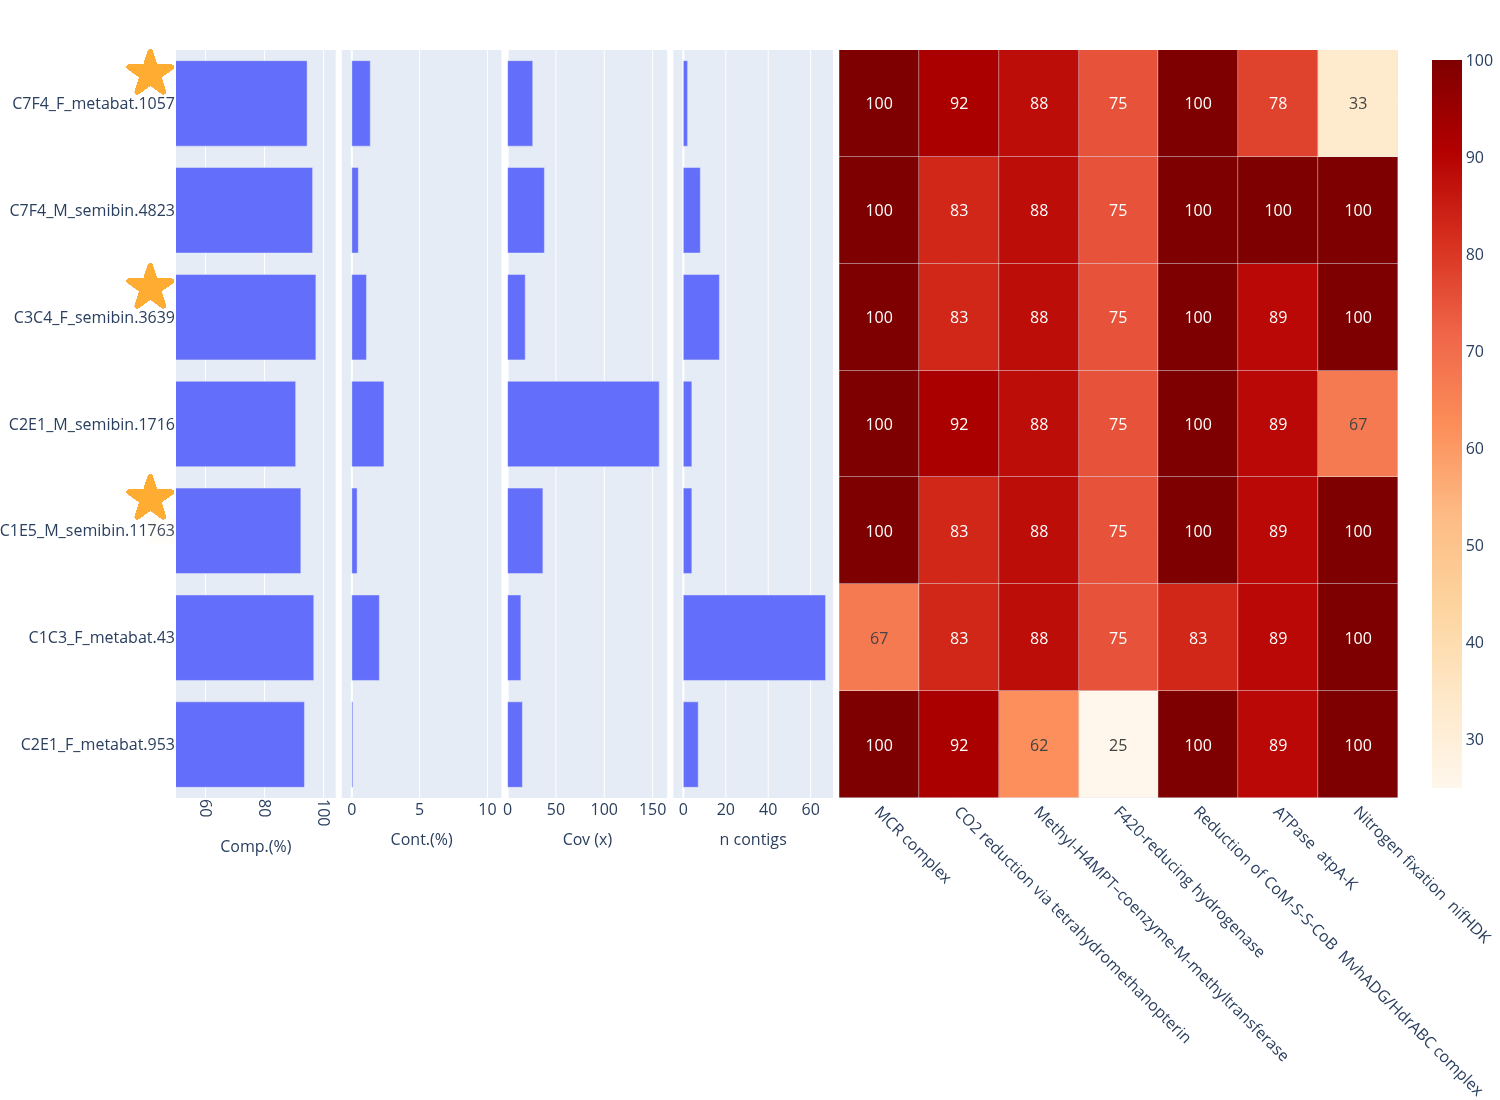
\includegraphics[width=\linewidth]{content-images/heatmap.png}
        \caption{\scriptsize CH$_4$ metabolism genes encoded by MCR-containing MAGs. MAG ID labels are shown on the left; only high-quality MAGs are included (minimum 90\% completeness, maximum 5\% contamination). Bar plots to the left of the heatmaps show MAG completeness, contamination, average read coverage per sample, and the number of contigs. Heatmap colors and values represent the completeness of each genetic component as a percentage. Genomes that we successfully assembled to singular circular contigs are annotated with stars.}
        \label{fig:heatmap}
    \end{figure}

    \vspace{-0.4cm}
    Three MAGs were further curated and successfully yield complete singular circular chromosome \ref{fig:heatmap}. The successful recovery of complete genomes of Bog-38 from NSPSF further proves their presence in the environment. This finding contrasts with their absence in another tropical peat soil environment, the Maludam National Park in Sarawak. 
    
    % \vspace{1.5em}

    % \begin{tcolorbox}
    % \lipsum[66]
    % \end{tcolorbox}
\end{multicols}

% \vspace{1.5em} % spacing before the full-width figure

% ---- Full-width TikZ block (outside multicols) ----
\begin{figure}[H]
    \vspace{-0.4cm}
    \centering
    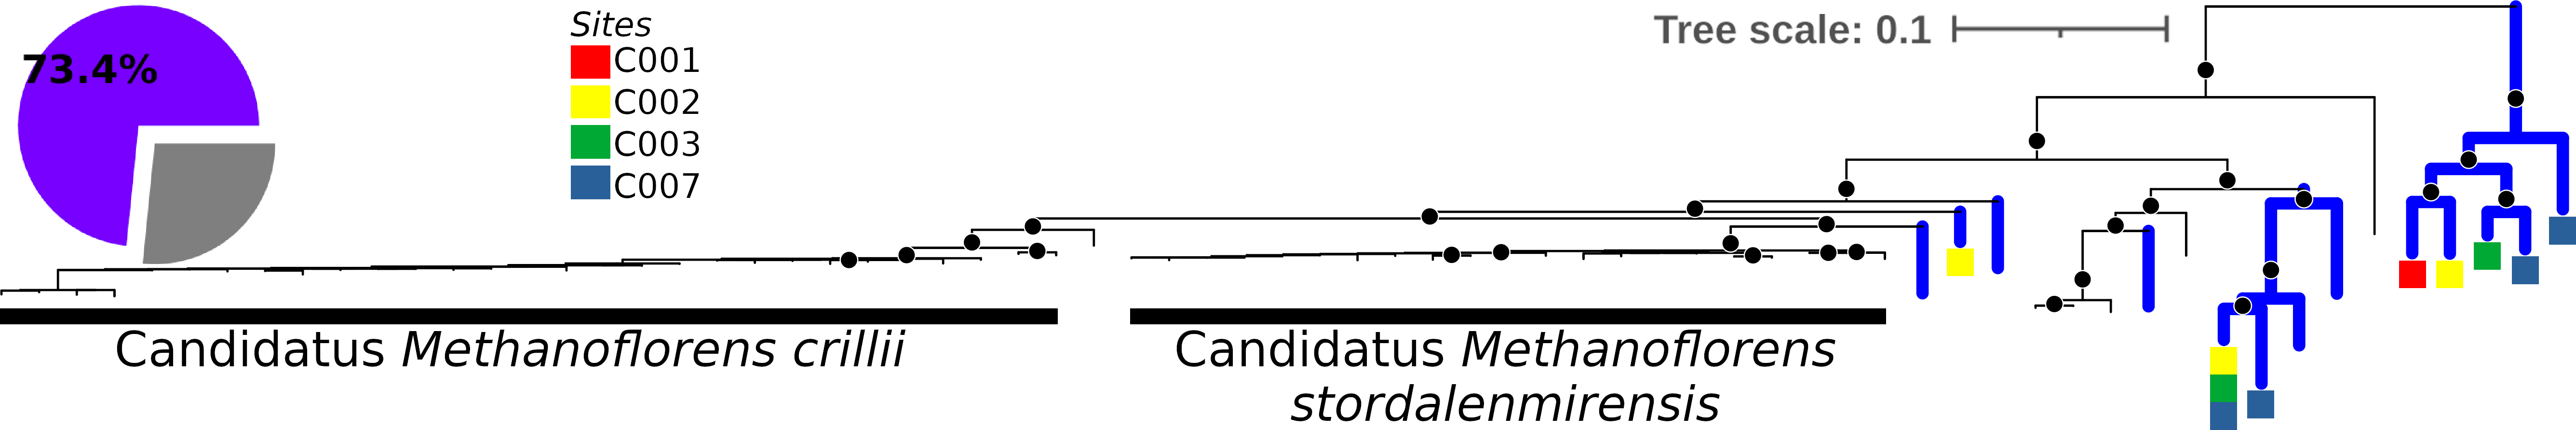
\includegraphics[width=\linewidth]{content-images/bog38_invert.png}
    \caption{\scriptsize Phylogenomic tree of archaeal class Bog-38. Candidatus \emph{Methanoflorens stordalenmirensis} and Candidatus \emph{Methanoflorens crillii} are indicated. Colored branches indicate MAGs that originate from the NSPSF dataset. Pie charts indicate increase in phylogenetic diversity from inclusion of NSPSF MAGs relative to currently available genomes in the public database (last accessed \nth{15} January 2025). Phylogenomic trees were rooted using outgroup c\_\_Methanomicrobia, which were removed from the final visualization. Bootstrap supports are indicated by black dots ranging from 90-100\%. Tree scale is 0.1. A MAG is deemed as present in a site if average coverage values are at least 10 in a site.}
    \label{fig:phylo}
\end{figure}  
}

%%%%%%%%%%%%%%%%%%%%%%%%%%%%%%%%%%%%%%%%%%%%%%%%%%%%%%%%%%%%%%%%%%%%%%%%%%%%%%
  \headerbox{\mytitlefont Conclusions}{name=conclusions,column=1,row=0,span=2, below=results }{
%%%%%%%%%%%%%%%%%%%%%%%%%%%%%%%%%%%%%%%%%%%%%%%%%%%%%%%%%%%%%%%%%%%%%%%%%%%%%%
  \mytextfont
  \footnotesize

\vspace{0.2em} % spacing before the full-width figure

% ---- Full-width TikZ block (outside multicols) ----
\begin{center}
\begin{tikzpicture}
    \node[anchor=west] at (0,0) {
        \begin{minipage}{0.15\textwidth}
        \centering
        \resizebox{\textwidth}{!}{
\includegraphics{homer_smart}}
        \end{minipage}
    };
    \node[anchor=west] at (2.5,0) { % Adjust X offset if needed
        \begin{minipage}{0.8\textwidth}
%         \begin{tcolorbox}
% Lorem ipsum dolor sit amet, consectetuer adipiscing elit. Aenean commodo ligula eget dolor. Aenean massa. Cum sociis natoque penatibus et magnis dis parturient montes, nascetur ridiculus mus. Donec quam felis, ultricies nec, pellentesque eu, pretium quis, sem. \textsuperscript{[3]}.
%         \end{tcolorbox}
        The detection of multiple Bog-38 MAGs in the NSPSF challenges the prevailing notion that this archaeal lineage is confined to Arctic and sub-Arctic peatlands. The presence of high-quality, complete MAGs encoding key methanogenesis genes such as the MCR and MTR complexes confirms their potential role in methane production within tropical ecosystems. Phylogenomic comparisons revealed that the tropical Bog-38 representatives form distinct clades, indicating previously unrecognized lineage diversification and suggesting that the biogeographical range and ecological niches of Bog-38 may be broader than currently understood, perhaps remained to be explored in tropical ecosystems.
        
        These findings lay the groundwork for future work to characterize the physiology, environmental responses, and ecological contributions of Bog-38 lineages in methane cycling across contrasting peatland ecosystems. More details available at: \url{github.com/ZarulHanifah/8thICMBB2025}
        \end{minipage}
    };
\end{tikzpicture}
\end{center}
}


%%%%%%%%%%%%%%%%%%%%%%%%%%%%%%%%%%%%%%%%%%%%%%%%%%%%%%%%%%%%%%%%%%%%%%%%%%%%%%
%   \headerbox{References}{headerColorOne=wasp_banner_dark, borderColor=wasp_banner_dark, name=results,column=0,row=0,span=1, below=methods }{
% %%%%%%%%%%%%%%%%%%%%%%%%%%%%%%%%%%%%%%%%%%%%%%%%%%%%%%%%%%%%%%%%%%%%%%%%%%%%%%
% 	\mytextfont
%   \small
\vspace{-0.5cm}
\fcolorbox{white}{white}{\hspace{-0.5cm}\parbox{0.1\linewidth}{\centering [1]}\parbox{1.3cm}{\includegraphics[trim=28mm 10mm 35mm 15mm,clip,width=0.8cm]{qracm}}\parbox{0.7\linewidth}{\footnotesize\smaller Five Challenges in Cloud-Enabled Intelligence and Control\\\tiny T. Abdelzaher, Y. Hao, K. Jayarajah, A. Misra, S. Yao, P. Skarin, D. Weerakoon and K. {\AA}rz{\'e}n\\ACM Transactions on Internet Technology, 2019}}\par\vspace{-0.4cm}
	
\fcolorbox{white}{white}{\hspace{-0.5cm}\parbox{0.1\linewidth}{\centering [2]}\parbox{1.3cm}{\includegraphics[trim=25mm 10mm 35mm 10mm,clip,width=0.8cm]{qredge1}}\parbox{0.7\linewidth}{\footnotesize\smaller Towards Mission-Critical Control at the Edge and Over 5G\\\tiny Per Skarin, William Tärneberg, Karl-Erik Årzén, Maria Kihl\\Best paper award, IEEE Services (EDGE), 2-7 July, 2018, San Fran., CA, USA}}\par\vspace{-0.25cm}
	
\fcolorbox{white}{white}{\hspace{-0.5cm}\parbox{0.1\linewidth}{\centering [5]}\parbox{1.3cm}{\includegraphics[trim=28mm 35mm 35mm 35mm,clip,width=0.8cm]{qrifac}}\parbox{0.7\linewidth}{\footnotesize\smaller Cloud-based model predictive control with variable horizon\\\tiny Per Skarin, Johan Eker, Karl-Erik Årzén\\Subm. to 21st World Congress of the International Federation of Automatic Control, 2020}}\par\vspace{-0.3cm}

% }

\headerbox{}{name=foottext, column=0, span=3, above=bottom, textborder=none,headerborder=none,boxheaderheight=0pt,boxColorOne=wasp_banner_dark}{\hfill 
\includegraphics[height=0.6cm]{content-images/acknowledgement.png}}


\end{poster}

\newpage

\label{Bibliography}
\lhead{\emph{Bibliography}}  % Change the left side page header to "Bibliography"
% \bibliographystyle{unsrtnat}  % Use the "unsrtnat" BibTeX style for formatting the Bibliography
\bibliographystyle{plainnat}
\bibliography{Bibliography}
\end{document}
